% Created 2023-02-17 Fri 17:48
% Intended LaTeX compiler: pdflatex
\documentclass[fontsize=11pt,paper=a4]{book}
\usepackage[utf8]{inputenc}
\usepackage[T1]{fontenc}
\usepackage{graphicx}
\usepackage{longtable}
\usepackage{wrapfig}
\usepackage{rotating}
\usepackage[normalem]{ulem}
\usepackage{amsmath}
\usepackage{amssymb}
\usepackage{capt-of}
\usepackage{hyperref}
\usepackage[linesnumbered]{algorithm2e}

\usepackage{amsthm}

\theoremstyle{plain}
\newtheorem{thm}{Theorem}
\newtheorem{corollary}[thm]{Corollary}
\newtheorem{lem}[thm]{Lemma}
\newtheorem{claim}[thm]{Claim}

\newenvironment{proof2}{%
\proof%
\renewcommand\qedsymbol{\blacksquare}
}{\endproof}

\theoremstyle{definition}
\newtheorem{defn}[thm]{Definition}
\newtheorem{notation}[thm]{Notation}

\theoremstyle{remark}
\newtheorem{remark}[thm]{Remark}

\usepackage{breqn}

\usepackage{mathrsfs}

\author{Mitja Daniel Krebs}
\date{\today}
\title{Congestion-Free Network Updates: Algorithms and Complexity}
\hypersetup{
 pdfauthor={Mitja Daniel Krebs},
 pdftitle={Congestion-Free Network Updates: Algorithms and Complexity},
 pdfkeywords={},
 pdfsubject={},
 pdfcreator={Emacs 28.2 (Org mode 9.6.1)}, 
 pdflang={English}}
\begin{document}

\maketitle
\tableofcontents

\begin{table}[htbp]
\caption{Table of notations}
\centering
\begin{tabular}{ll}
\hyperref[org5611292]{\(b(v,P)\)} & The \(P\)-block containing vertex \(v\)\\[0pt]
\hyperref[org6e70c40]{\(B^P(G)\)} & The set of \(P\)-blocks\\[0pt]
\hyperref[org2d9ed81]{\(B(G)\)} & The set of blocks\\[0pt]
\hyperref[orge8cadd8]{\(\mathcal{B}(b)\)} & The round in which block \(b\) is updated\\[0pt]
\hyperref[org99dba3a]{\(\mathcal{B}(v,P)\)} & The round in which block \(b(v,P)\) is updated\\[0pt]
\hyperref[org56dcc69]{\(B_i\)} & The set of blocks updated before or in the \(i\)-th round\\[0pt]
 & \\[0pt]
\end{tabular}
\end{table}

\part{Preliminaries}
\label{sec:org8be0682}

\begin{notation}
For a flow pair \(P\) and a vertex \(v\in V(P)\), \(b(v,P)\) denotes the \(P\)-block containing \(v\).
\label{org5611292}
\end{notation}

\begin{notation}
For an update flow network \(G\) and a flow pair \(P\), \(B^P(G)\) denotes the set of \(P\)-blocks.
\label{org6e70c40}
\end{notation}

\begin{notation}
For an update flow network \(G\), \(B(G)=\bigcup_{P\in\mathcal{P}}B^P(G)\)
\label{org2d9ed81}
\end{notation}

\begin{defn}
A \emph{block sequence} \(\mathcal{B}=(\mathscr{B}_1,\dots,\mathscr{B}_{\ell})\) is an ordered partition of the set of blocks.
\label{org85175c2}
\end{defn}

\begin{notation}
For a block sequence \(\mathcal{B}=(\mathscr{B}_1,\dots,\mathscr{B}_{\ell})\) and a block \(b\), \(\mathcal{B}(b)\) denotes the index \(i\in[\ell]\) such that \(b\) is contained in \(\mathscr{B}_i\).
\label{orge8cadd8}
\end{notation}

\begin{notation}
For a block sequence \(\mathcal{B}=(\mathscr{B}_1,\dots,\mathscr{B}_{\ell})\), a flow pair \(P\), and a vertex \(v\in V(P)\), \(\mathcal{B}(v,P)=\mathcal{B}(b(v,P))\) denotes the index \(i\in[\ell]\) such that block \(b(v,P)\) is contained in \(\mathscr{B}_i\).
\label{org99dba3a}
\end{notation}

\begin{notation}
For a block sequence \(\mathcal{B}=(\mathscr{B}_1,\dots,\mathscr{B}_{\ell})\) and an index \(i\in[\ell]\), \(B_i=\bigcup_{j\leq i}\mathscr{B}_j\) denotes the set of blocks updated before or in the \(i\)-th round.
\label{org56dcc69}
\end{notation}

\begin{defn}
Let \(\mathcal{B}=(\mathscr{B}_1,\dots,\mathscr{B}_{\ell})\) be a block sequence.
For a flow pair \(P\), an edge \((u,v)\in E(P^o\cup P^u)\), and an index \(i\in[\ell]\), the \emph{activation label} \(\alpha_P((u,v),B_i)\) is defined as follows:
\[\alpha_P((u,v),B_i)=
\begin{cases}
\mathrm{active} & \text{if }(u,v)\in E(P^o)\text{ and }b(u,P)\notin B_i\\
\mathrm{active} & \text{if }(u,v)\in E(P^u)\text{ and }b(u,P)\in B_i\\
\mathrm{inactive} & \text{otherwise}.
\end{cases}\]
\label{org5295a66}
\end{defn}

\begin{lem}
Let \(\mathcal{B}=(\mathscr{B}_1,\dots,\mathscr{B}_{\ell})\) be a block sequence, \(P\) be a flow pair, \((u,v)\in E(P^o\cup P^u)\), and \(i\in[\ell]\).
Then:

\begin{enumerate}
\item If \((u,v)\in E(P^o\setminus P^u)\), then
\[\alpha_P((u,v),B_i)=
   \begin{cases}
   \mathrm{active} & i<\mathcal{B}(u,P)\\
   \mathrm{inactive} & i\geq\mathcal{B}(u,P).
   \end{cases}\]

\item If \((u,v)\in E(P^o\cap P^u)\), then \(\alpha_P((u,v)B_i)=\mathrm{active}\).

\item If \((u,v)\in E(P^u\setminus P^o)\), then
\[\alpha_P((u,v),B_i)=
   \begin{cases}
   \mathrm{active} & i\geq\mathcal{B}(u,P)\\
   \mathrm{inactive} & i<\mathcal{B}(u,P).
   \end{cases}\]
\end{enumerate}
\label{org6b790d7}
\end{lem}

\begin{defn}
A block sequence \(\mathcal{B}=(\mathscr{B}_1,\dots,\mathscr{B}_{\ell})\) is \emph{feasible} if for every edge \(e\) and every index \(i\in[\ell]\),
\begin{equation}
c(e)\(\ge \sum\)\textsubscript{P\(\in\)\mathcal{P}:\(\alpha\)\textsubscript{P}(e,B\textsubscript{i-1})=\mathrm{active}\text{ or }\(\alpha\)\textsubscript{P}(e,B\textsubscript{i})=\mathrm{active}}d\textsubscript{P},
\label{org8070f03}
\end{equation}
where we define \(\mathscr{B}_0=\emptyset\).
\label{orge1a853d}
\end{defn}

\begin{remark}
Let \(G\) be an update flow network with unit demand equal to \(1\), that is, \(d_P=1\) for every flow pair \(P\), and let \(\mathcal{B}=(\mathscr{B}_1,\dots,\mathscr{B}_{\ell})\) be a block sequence.
Then, for every edge \(e\) and every index \(i\in[\ell]\), capacity constraint \ref{org8070f03} simplifies to:
\begin{align*}
c(e)
&\geq\sum_{P\in\mathcal{P}:\alpha_P(e,B_{i-1})=\mathrm{active}\text{ or }\alpha_P(e,B_i)=\mathrm{active}}d_P\\
&=\sum_{P\in\mathcal{P}:\alpha_P(e,B_{i-1})=\mathrm{active}\text{ or }\alpha_P(e,B_i)=\mathrm{active}}1\\
&=\lvert\{P\in\mathcal{P}\mid\alpha_P(e,B_{i-1})=\mathrm{active}\text{ or }\alpha_P(e,B_i)=\mathrm{active}\}\rvert.
\end{align*}
\label{org31f9978}
\end{remark}

\begin{corollary}
There is a feasible block sequence iff there is a feasible update sequence.
\label{orged5cf81}
\end{corollary}

\part{\(\textbf{NP}\)-Hardness for \(k=3\)}
\label{sec:org2cb88e8}

The goal of this section is to prove the following theorem.

\begin{thm}
The \(k\)-network flow update problem is \(\textbf{NP}\)-hard for \(k=3\).
\label{org7f47b71}
\end{thm}

We will prove this theorem in two steps. First, we will prove the following theorem.

\begin{thm}
The \(k\)-network flow update problem, where every edge is used by at most three flow pairs, is \(\textbf{NP}\)-hard for \(k=10\).
\label{orgea6d1e6}
\end{thm}

Then, we will (repeatedly) apply the following lemma to the flow update network we will have constructed in the proof of Theorem \ref{orgea6d1e6} to reduce the number of flow pairs from \(10\) to \(3\).

\begin{lem}
Hehe.
\label{orgc1908b1}
\end{lem}

\chapter{\(\textbf{NP}\)-Hardness for the Special Case}
\label{sec:org8eb8156}

The proof of Theorem \ref{orgea6d1e6} is via reduction from \(\textsf{4-SAT}\) and is based on the \(\textbf{NP}\)-hardness proof for \(k=6\) in (Amiri, Saeed A. and Dudycz, Szymon and Parham, Mahmoud and Schmid, Stefan and Wiederrecht, Sebastian, 2019).

\section{The Reduction}
\label{sec:org0ef05a0}

Let \(C\) be a 4CNF formula with \(n\) variables \(x_1,\dots,x_n\) and \(m\) clauses \(C_1,\dots,C_m\).
W.l.o.g. every variable occurs both positively and negatively (otherwise, if a variable \(x_j\) occurs only positively (negatively), we can assign \(1\) (\(0\)) to \(x_j\) and remove all clauses containing literal \(x_j\) (\(\bar{x}_j\))).
We construct the corresponding update flow network \(G\) as follows.
First, we introduce a \emph{clause gadget} for each clause and a \emph{variable gadget} for each variable.
Then, we connect the variable and clause gadgets.
Finally, we take the remaining steps necessary to ensure that \(G\) is indeed a feasible update flow network.

\paragraph{Clause gadgets.}
Let \(C_i=(l_{i_1}\vee l_{i_2}\vee l_{i_3}\vee l_{i_4})\) be a clause.
We construct the corresponding clause gadget \(C^i\) as follows.
The idea is to model the syntax tree for \(C_i\) depicted in Figure \ref{fig:org407a649}.

\begin{figure}[htbp]
\centering
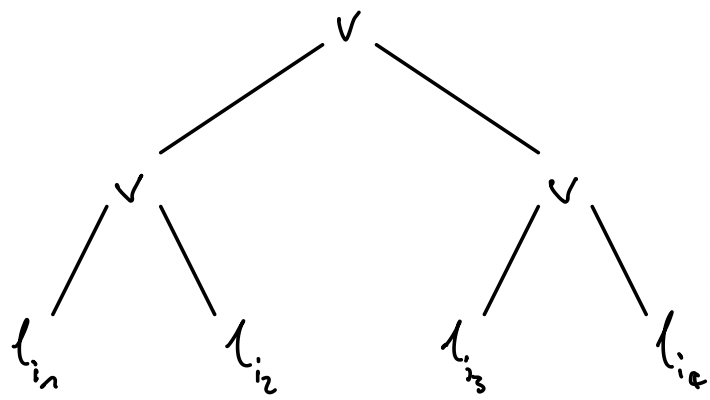
\includegraphics[width=.9\linewidth]{../assets/Screen Shot 2023-02-14 at 15.05.37.png}
\caption{\label{fig:org407a649}A syntax tree for clause \((l_{i_1}\vee l_{i_2}\vee l_{i_3}\vee l_{i_4})\)}
\end{figure}

For the root operator node, we introduce a \emph{clause vertex} \(u^i\) which is used by three flow pairs \(L,R,B\).
The idea is to guarantee that clause \(C_i\) is satisfied iff block \(b(u^i,L)\) is updated before block \(b(u^i,B)\) or block \(b(u^i,R)\) is updated before \(b(u^i,B)\).
Equivalently, \(b(u^i,B)\) cannot be updated unless at least one of \(b(u^i,L),b(u^i,R)\) has been updated.
Intuitively, if \(b(u^i,L)\) (\(b(u^i,R)\)) is updated before \(b(u^i,B)\), then the \(\textbf{L}\)eft half \((l_{i_1}\vee l_{i_2})\) (\(\textbf{R}\)ight half \((l_{i_3}\vee l_{i_4})\)) of \(C_i\) is satisfied.

Similarly, for the intermediate operator nodes of the syntax tree, we introduce clause vertices \(u_{1,2}^i,u_{3,4}^i\), where \(u_{1,2}^i\) corresponds to \((l_{i_1}\vee l_{i_2})\) and \(u_{3,4}^i\) corresponds to \((l_{i_3}\vee l_{i_4})\).
Both clause vertices are used by flow pairs \(\tilde{L},\tilde{R},\tilde{B}\) such that if \(b(u_{1,2}^i,\tilde{L})\) (\(b(u_{1,2}^i,\tilde{R})\)) is updated before \(b(u_{1,2},\tilde{B})\), then the left half \(l_{i_1}\) (right half \(l_{i_2}\)) of \((l_{i_1}\vee l_{i_2})\) is satisfied, and analogously for \(u_{3,4}^i\).

Moreover, for the operand nodes of the syntax tree, we introduce \emph{literal vertices} \(u_1^i,u_2^i,u_3^i,u_4^i\).

Finally, for every branch from a parent node to its left (right) child node, we add an edge to either \(L\) (\(R\)) (if the parent node is \(u^i\)) or \(\tilde{L}\) (\(\tilde{R}\)) (if the parent node is \(u_{1,2}^i\) or \(u_{3,4}^i\)).

We now proceed with the detailed specification of clause gadget \(C^i\) (see Figure \ref{fig:org5b5792f}).

\begin{figure}[htbp]
\centering
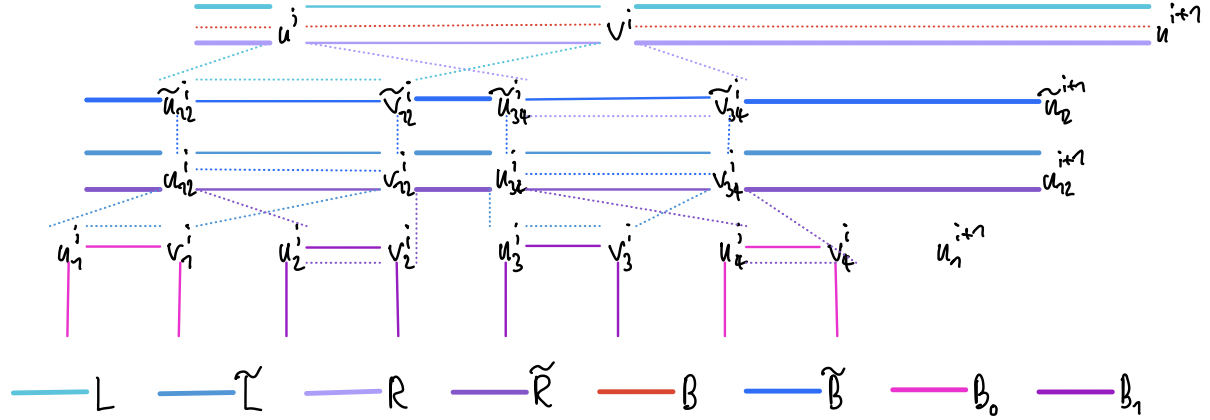
\includegraphics[width=.9\linewidth]{../assets/Screen Shot 2023-02-14 at 15.07.03.png}
\caption{\label{fig:org5b5792f}Clause gadget \(C^i\)}
\end{figure}

We introduce six flow pairs \(L,R,B,\tilde{L},\tilde{R},\tilde{B}\), each with demand \(1\).

For the clause vertices, we introduce two vertices \(u^i,v^i\) and add edge \((u^i,v^i)\) to flows \(L^o,R^o,B^u\).
Similarly, we introduce vertices \(u_{1,2}^i,v_{1,2}^i,u_{3,4}^i,v_{3,4}^i\) and add edges \((u_{1,2}^i,v_{1,2}^i),(u_{3,4}^i,v_{3,4}^i)\) to flows \(\tilde{L}^o,\tilde{R}^o,\tilde{B}^u\).

For the literal vertices, we introduce vertices \(u_1^i,v_1^i,u_2^i,v_2^i,u_3^i,v_3^i,u_4^i,v_4^i\) and add edges \((u_1^i,v_1^i),(u_3^i,v_3^i)\) to flow \(\tilde{L}^u\) and \((u_2^i,v_2^i),(u_4^i,v_4^i)\) to \(\tilde{R}^u\).

Moreover, we introduce auxiliary vertices \(\tilde{u}_{1,2}^i,\tilde{v}_{1,2}^i,\tilde{u}_{3,4}^i,\tilde{v}_{3,4}^i\) and add edge \((\tilde{u}_{1,2}^i,\tilde{v}_{1,2}^i)\) to flows \(\tilde{L}^u,\tilde{B}^o\) and \((\tilde{u}_{3,4}^i,\tilde{v}_{3,4}^i)\) to \(\tilde{R}^u,\tilde{B}^o\).

Finally, we add the following edges to connect clause gadget \(C^i\):

\begin{itemize}
\item \((u^i,\tilde{u}_{1,2}^i),(\tilde{v}_{1,2}^i,v^i)\) to \(L^u\)
\item \((u^i,\tilde{u}_{3,4}^i),(\tilde{v}_{3,4}^i,v^i)\) to \(R^u\)
\item \((v_{1,2}^i,u_{3,4}^i)\) to \(\tilde{L}^o,\tilde{L}^u,\tilde{R}^o,\tilde{R}^u\)
\item \((u_{1,2}^i,u_1^i),(v_1^i,v_{1,2}^i),(u_{3,4}^i,u_3^i),(v_3^i,v_{3,4}^i)\) to \(\tilde{L}^u\)
\item \((u_{1,2}^i,u_2^i),(v_2^i,v_{1,2}^i),(u_{3,4}^i,u_4^i),(v_4^i,v_{3,4}^i)\) to \(\tilde{R}^u\)
\item \((\tilde{v}_{1,2}^i,\tilde{u}_{3,4}^i)\) to \(\tilde{B}^o,\tilde{B}^u\)
\item \((\tilde{u}_{1,2}^i,u_{1,2}^i),(v_{1,2}^i,\tilde{v}_{1,2}^i),(\tilde{u}_{3,4}^i,u_{3,4}^i),(v_{3,4}^i,\tilde{v}_{3,4}^i)\) to \(\tilde{B}^u\)
\end{itemize}

\paragraph{Variable gadgets.}
For every variable \(x_j\), we construct the corresponding variable gadget \(X^j\) as follows.
We introduce a \emph{variable vertex} \(x^j\) which is used by three flow pairs \(X,\bar{X},B\). The idea is to guarantee the following:

\begin{enumerate}
\item If block \(b(x^j,X)\) is updated before block \(b(x^j,B)\), then variable \(x_j\) is assigned \(1\).
\item If block \(b(x^j,\bar{X})\) is updated before \(b(x^j,B)\), then \(x_j\) is assigned \(0\).
\item Not both \(b(x^j,X)\) and \(b(x^j,\bar{X})\) can be updated before \(b(x^j,B)\).
\end{enumerate}

We now proceed with the detailed specification of variable gadget \(X^j\) (see Figure \ref{fig:org59b2466}).

\begin{figure}[htbp]
\centering
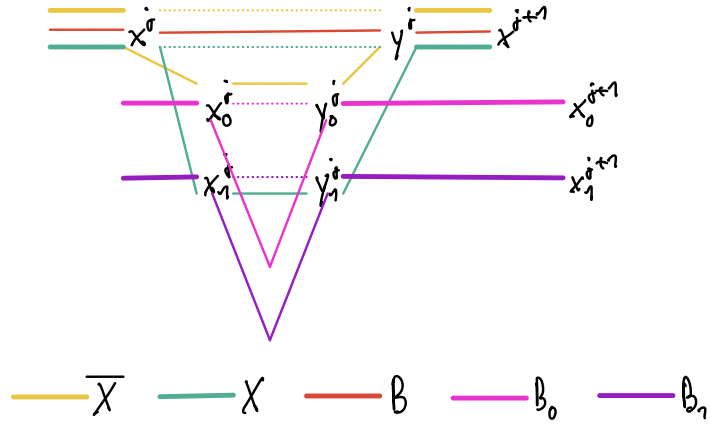
\includegraphics[width=.9\linewidth]{../assets/Screen Shot 2023-02-14 at 15.06.35.png}
\caption{\label{fig:org59b2466}Variable gadget \(X^j\)}
\end{figure}

We introduce two flow pairs \(X,\bar{X}\), each with demand \(1\).
For the variable vertices, we introduce vertices \(x^j,y^j\) and add edge \((x^j,y^j)\) to flows \(X^u,\bar{X}^u,B^o\).
Moreover, we introduce auxiliary vertices \(x_0^j,y_0^j,x_1^j,y_1^j\) and add edge \((x_0^j,y_0^j)\) to flow \(\bar{X}^o\) and \((x_1^j,y_1^j)\) to \(X^o\).
Finally, to connect variable gadget \(X^j\), we add edges \((x^j,x_0^j),(y_0^j,y^j)\) to flow \(\bar{X}^o\) and \((x^j,x_1^j),(y_1^j,y^j)\) to \(X^o\).

\paragraph{Connecting variable with clause gadgets.}
For every \(j\in[n]\) and every \(i\in[m]\), we connect variable gadget \(X^j\) to clause gadget \(C^i\) if variable \(x_j\) occurs in clause \(C_i\).
More precisely, we introduce two flow pairs \(B_0,B_1\), each with demand \(1\), such that \(B_0\) (\(B_1\)) connects vertex \(x_0^j\) (\(x_1^j\)) to all literal vertices corresponding to literal \(\bar{x}_j\) (\(x_j\)).

More formally, for every \(j\in[n]\), let \(P_j=\{p_1^j,\dots,p_{\ell_j}^j\}\) denote the set of indices of the clauses containing literal \(x_j\) and \(\bar{P}_j=\{\bar{p}_1^j,\dots,p_{\ell'_j}^j\}\) denote the set of indices of the clauses containing literal \(\bar{x}_j\).
Moreover, for every \(j\in[n]\) and every \(i\in[m]\), let \(\pi(i,j)\) denote the position of literal \(x_j\) in clause \(C_i\) and \(\bar{\pi}(i,j)\) denote the position of literal \(\bar{x}_j\) in \(C_i\).
For every \(j\in[n]\), we add the following edges:

\begin{itemize}
\item \((x_0^j,u_{\bar{\pi}(\bar{p}_1^j,j)}^{\bar{p}_1^j})\), \((u_{\bar{\pi}(\bar{p}_{\ell}^j,j)}^{\bar{p}_{\ell}^j},v_{\bar{\pi}(\bar{p}_{\ell}^j,j)}^{\bar{p}_{\ell}^j})\) for every \(\ell\in[\ell'_j]\), \((v_{\bar{\pi}(\bar{p}_{\ell}^j,j)}^{\bar{p}_{\ell}^j},u_{\bar{\pi}(\bar{p}_{\ell+1}^j,j)}^{\bar{p}_{\ell+1}^j})\) for every \(\ell\in[\ell'_j-1]\), and \((v_{\bar{\pi}(\bar{p}_{\ell'_j}^j,j)}^{\bar{p}_{\ell'_j}^j},y_0^j)\) to \(B_0^o\)
\item \((x_1^j,u_{\pi(p_1^j,j)}^{p_1^j})\), \((u_{\pi(p_{\ell}^j,j)}^{p_{\ell}^j},v_{\pi(p_{\ell}^j,j)}^{p_{\ell}^j})\) for every \(\ell\in[\ell_j]\), \((v_{\pi(p_{\ell}^j,j)}^{p_{\ell}^j},u_{\pi(p_{\ell+1}^j,j)}^{p_{\ell+1}^j})\) for every \(\ell\in[\ell_j-1]\), and \((v_{\pi(p_{\ell_j}^j,j)}^{p_{\ell_j}^j},y_1^j)\) to \(B_1^o\)
\end{itemize}

\paragraph{Completing the update flow network.}
We introduce vertices \(s,t\) and create (\(s,t\))-paths for all flows by adding the following edges:

\begin{itemize}
\item \((s,u^1),(v^m,t)\) to \(L^o,L^u,R^o,R^u\)
\item \((v^i,u^{i+1})\) for every \(i\in[m-1]\) to \(L^o,L^u,R^o,R^u,B^u\)
\item \((s,u_{1,2}^1)\), \((v_{3,4}^i,u_{1,2}^{i+1})\) for every \(i\in[m-1]\), and \((v_{3,4}^m,t)\) to \(\tilde{L}^o,\tilde{L}^u,\tilde{R}^o,\tilde{R}^u\)
\item \((s,\tilde{u}_{1,2}^1)\), \((\tilde{v}_{3,4}^i,\tilde{u}_{1,2}^{i+1})\) for every \(i\in[m-1]\), and \((\tilde{v}_{3,4}^m,t)\) to \(\tilde{B}^o,\tilde{B}^u\)
\item \((s,x^1),(y^n,t)\) to \(X^o,X^u,\bar{X}^o,\bar{X}^u,B^o,B^u\)
\item \((y^j,x^{j+1})\) for every \(j\in[n-1]\) to \(X^o,X^u,\bar{X}^o,\bar{X}^u,B^o\)
\item \((x^1,u^1),(v^m,y^n)\) to \(B^u\)
\item \((s,x_0^1)\), \((y_0^j,x_0^{j+1})\) for every \(j\in[n-1]\), and \((y_0^n,t)\) to \(B_0^o,B_0^u\)
\item \((s,x_1^1)\), \((y_1^j,x_1^{j+1})\) for every \(j\in[n-1]\), and \((y_1^n,t)\) to \(B_1^o,B_1^u\)
\end{itemize}

See Figure \ref{fig:orga75fbf5} for the complete update flow network.
See Table \ref{tab:org0792dc7} for all (\(s,t\))-flows.

\begin{figure}[htbp]
\centering
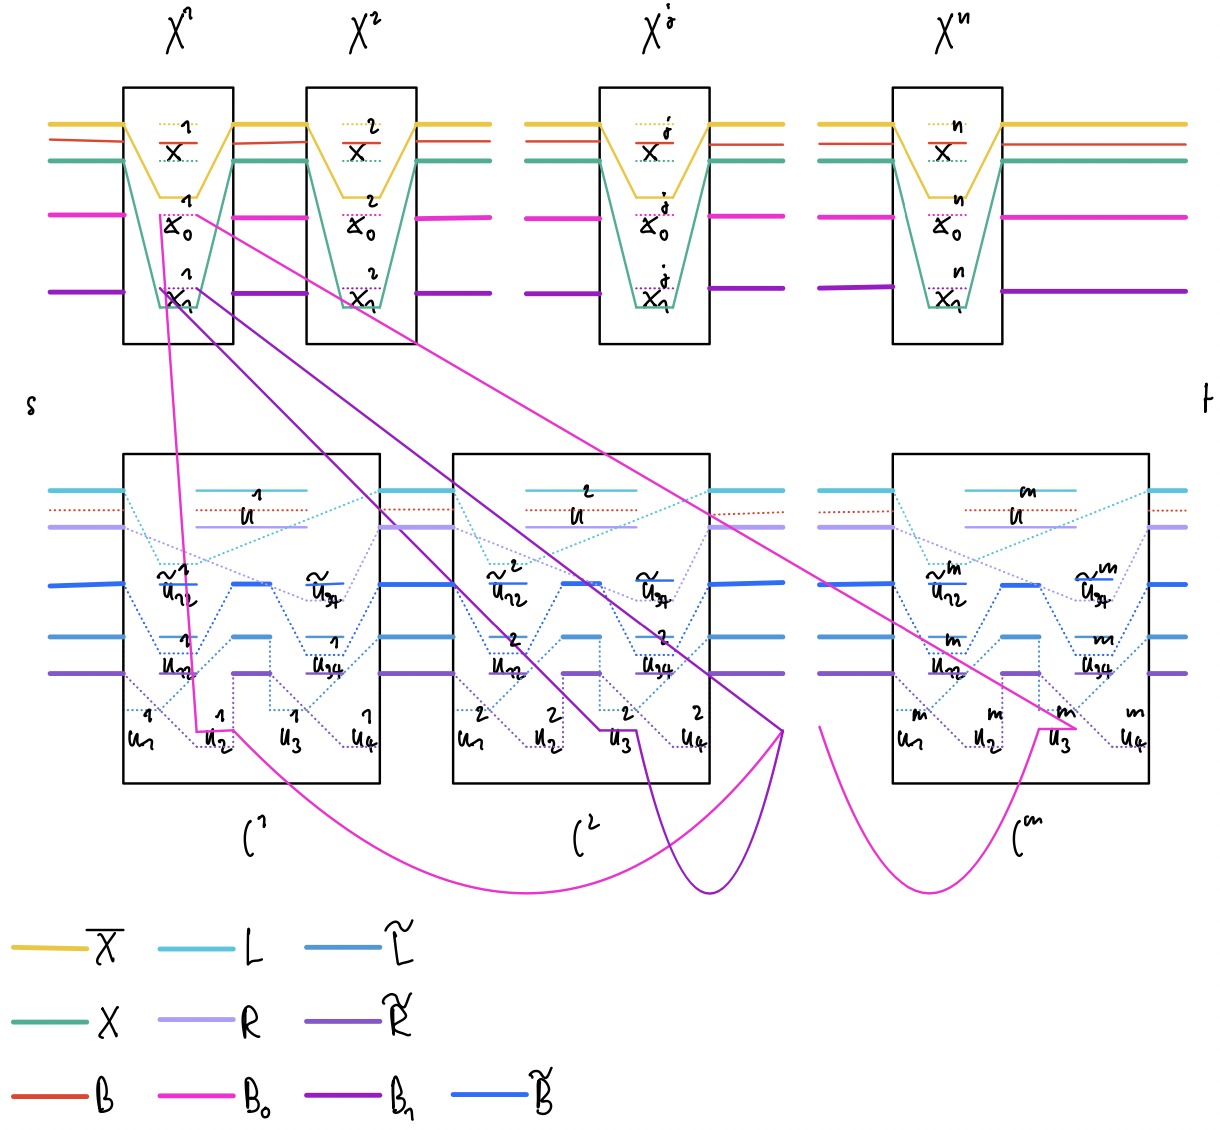
\includegraphics[width=.9\linewidth]{../assets/Screen Shot 2023-02-14 at 15.08.01.png}
\caption{\label{fig:orga75fbf5}The update flow network}
\end{figure}

\begin{table}[htbp]
\caption{\label{tab:org0792dc7}All (\(s,t\))-flows}
\centering
\begin{tabular}{ll}
Flow & (\(s,t\))-path\\[0pt]
\hline
\(\bar{X}^o\) & \(s,x^1,x_0^1,y_0^1,y^1,x^2,\dots,y^n,t\)\\[0pt]
\(\bar{X}^u\) & \(s,x^1,y^1,x^2,\dots,y^n,t\)\\[0pt]
\hline
\(L^o\) & \(s,u^1,v^1,u^2,\dots,v^m,t\)\\[0pt]
\(L^u\) & \(s,u^1,\tilde{u}_{1,2}^1,\tilde{v}_{1,2}^1,v^1,u^2,\dots,v^m,t\)\\[0pt]
\hline
\(\tilde{L}^o\) & \(s,u_{1,2}^1,v_{1,2}^1,u_{3,4}^1,v_{3,4}^1,u_{1,2}^2,\dots,v_{3,4}^m,t\)\\[0pt]
\(\tilde{L}^u\) & \(s,u_{1,2}^1,u_1^1,v_1^1,v_{1,2}^1,u_{3,4}^1,u_3^1,v_3^1,v_{3,4}^1,u_{1,2}^2,\dots,v_{3,4}^m,t\)\\[0pt]
\hline
\(X^o\) & \(s,x^1,x_1^1,y_1^1,y^1,x^2,\dots,y^n,t\)\\[0pt]
\(X^u\) & \(s,x^1,y^1,x^2,\dots,y^n,t\)\\[0pt]
\hline
\(R^o\) & \(s,u^1,v^1,u^2,\dots,v^m,t\)\\[0pt]
\(R^u\) & \(s,u^1,\tilde{u}_{3,4}^1,\tilde{v}_{3,4}^1,v^1,u^2,\dots,v^m,t\)\\[0pt]
\hline
\(\tilde{R}^o\) & \(s,u_{1,2}^1,v_{1,2}^1,u_{3,4}^1,v_{3,4}^1,u_{1,2}^2,\dots,v_{3,4}^m,t\)\\[0pt]
\(\tilde{R}^u\) & \(s,u_{1,2}^1,u_2^1,v_2^1,v_{1,2}^1,u_{3,4}^1,u_4^1,v_4^1,v_{3,4}^1,u_{1,2}^2,\dots,v_{3,4}^m,t\)\\[0pt]
\hline
\(B^o\) & \(s,x^1,y^1,x^2,\dots,y^n,t\)\\[0pt]
\(B^u\) & \(s,x^1,u^1,v^1,u^2,\dots,v^m,y^n,t\)\\[0pt]
\hline
\(\tilde{B}^o\) & \(s,\tilde{u}_{1,2}^1,\tilde{v}_{1,2}^1,\tilde{u}_{3,4}^1,\tilde{v}_{3,4}^1,\tilde{u}_{1,2}^2,\dots,\tilde{v}_{3,4}^m,t\)\\[0pt]
\(\tilde{B}^u\) & \(s,\tilde{u}_{1,2}^1,u_{1,2}^1,v_{1,2}^1,\tilde{v}_{1,2}^1,\tilde{u}_{3,4}^1,u_{3,4}^1,v_{3,4}^1,\tilde{v}_{3,4}^1,\tilde{u}_{1,2}^2,\dots,\tilde{v}_{3,4}^m,t^\)\\[0pt]
\hline
\(B_0^o\) & \(s,x_0^1,u_{\bar{\pi}(\bar{p}_1^1,1)}^{\bar{p}_1^1},v_{\bar{\pi}(\bar{p}_1^1,1)}^{\bar{p}_1^1},u_{\bar{\pi}(\bar{p}_2^1,1)}^{\bar{p}_2^1},\dots,v_{\bar{\pi}(\bar{p}_{l'_1}^1,1)}^{\bar{p}_{l'_1}^1},y_0^1,x_0^2,\dots,y_0^n,t\)\\[0pt]
\(B_0^u\) & \(s,x_0^1,y_0^1,x_0^2,\dots,y_0^n,t\)\\[0pt]
\hline
\(B_1^o\) & \(s,x_1^1,u_{\pi(p_1^1,1)}^{p_1^1},v_{\pi(p_1^1,1)}^{p_1^1},u_{\pi(p_2^1,1)}^{p_2^1},\dots,v_{\pi(p_{l_1}^1,1)}^{p_{l_1}^1},y_0^1,x_0^2,\dots,y_0^n,t\)\\[0pt]
\(B_1^u\) & \(s,x_1^1,y_1^1,x_1^2,\dots,y_1^n,t\)\\[0pt]
 & \\[0pt]
\end{tabular}
\end{table}

Edge capacities are defined as follows.

\begin{itemize}
\item We set the capacity to \(2\) for edges \((u^i,v^i),(u_{1,2}^i,v_{1,2}^i),(u_{3,4}^i,v_{3,4}^i),(x^j,y^j)\) for every \(i\in[m]\) and every \(j\in[n]\).
\item We set the capacity to \(1\) for edges \((u_1^i,v_1^i),(u_2^i,v_2^i),(u_3^i,v_3^i),(u_4^i,v_4^i),(\tilde{u}_{1,2}^i,\tilde{v}_{1,2}^i),(\tilde{u}_{3,4}^i,\tilde{v}_{3,4}^i),(x_0^j,y_0^j),(x_1^j,y_1^j)\) for every \(i\in[m]\) and every \(j\in[n]\).
\item All remaining edge capacities are set to \(10\), that is, the number of flow pairs, which equals the sum of all demands.
\end{itemize}

We remark that vertices \(\tilde{u}_{1,2}^i,\tilde{v}_{1,2}^i,\tilde{u}_{3,4}^i,\tilde{v}_{3,4}^i\) are not necessary for this proof.
Instead, we could directly connect clause vertices \(u^i,u_{1,2}^i\) via flow pair \(L\) and \(u^i,u_{3,4}^i\) via \(R\). Similarly, vertices \(x_0^j,y_0^j,x_1^j,y_1^j\) as well as flow pairs \(B_0,B_1\) are not necessary.
We could instead directly connect variable vertex \(x^j\) to literal vertex, say \(u_1^i\), via \(X\) (\(\bar{X}\)) if \(l_{i_1}=x_j\) (\(l_{i_1}=\bar{x}_j\)).
The vertices and flow pairs are necessary, however, for the proof of Theorem \ref{org7f47b71}.

Let us quickly verify that \(G\) is indeed a feasible update flow network.

\begin{itemize}
\item[{$\square$}] Feasibility.
\end{itemize}

\begin{table}[htbp]
\caption{\label{tab:orgd3cec77}All blocks grouped by flow pair}
\centering
\begin{tabular}{lll}
\(P\) & \(V(P^o\cap P^u)\) ordered w.r.t. \(\leq_{P^o\cup P^u}\) & \(B^P(G)\)\\[0pt]
\hline
\(\bar{X}\) & \(s,x^1,y^1,x^2,\dots,y^n,t\) & \(\{s,x^1\}\),\\[0pt]
 &  & \(\{x^j,x_0^j,y_0^j,y^j\},j\in[n]\),\\[0pt]
 &  & \(\{y^j,x^{j+1}\},j\in[n-1]\),\\[0pt]
 &  & \(\{y^n,t\}\)\\[0pt]
\hline
\(L\) & \(s,u^1,v^1,u^2,\dots,v^m,t\) & \(\{s,u^1\}\),\\[0pt]
 &  & \(\{u^i,\tilde{u}_{1,2}^i,\tilde{v}_{1,2}^i,v^i\},i\in[m]\),\\[0pt]
 &  & \(\{v^i,u^{i+1}\},i\in[m-1]\),\\[0pt]
 &  & \(\{v^m,t\}\)\\[0pt]
\hline
\(\tilde{L}\) & \(s,u_{1,2}^1,v_{1,2}^1,u_{3,4}^1,v_{3,4}^1,u_{1,2}^2,\dots,v_{3,4}^m,t\) & \(\{s,u_{1,2}^1\}\),\\[0pt]
 &  & \(\{u_{1,2}^i,u_1^i,v_1^i,v_{1,2}^i\},i\in[m]\),\\[0pt]
 &  & \(\{v_{1,2}^i,u_{3,4}^i\},i\in[m]\),\\[0pt]
 &  & \(\{u_{3,4}^i,u_3^i,v_3^i,v_{3,4}^i\},i\in[m]\),\\[0pt]
 &  & \(\{v_{3,4}^i,u_{1,2}^{i+1}\},i\in[m-1]\),\\[0pt]
 &  & \(\{v_{3,4}^m,t\}\)\\[0pt]
\hline
\(X\) & \(s,x^1,y^1,x^2,\dots,y^n,t\) & \(\{s,x^1\}\),\\[0pt]
 &  & \(\{x^j,x_1^j,y_1^j,y^j\},j\in[n]\),\\[0pt]
 &  & \(\{y^j,x^{j+1}\},j\in[n-1]\),\\[0pt]
 &  & \(\{y^n,t\}\)\\[0pt]
\hline
\(R\) & \(s,u^1,v^1,u^2,\dots,v^m,t\) & \(\{s,u^1\}\),\\[0pt]
 &  & \(\{u^i,\tilde{u}_{3,4}^i,\tilde{v}_{3,4}^i,v^i\},i\in[m]\),\\[0pt]
 &  & \(\{v^i,u^{i+1}\},i\in[m-1]\),\\[0pt]
 &  & \(\{v^m,t\}\)\\[0pt]
\hline
\(\tilde{R}\) & \(s,u_{1,2}^1,v_{1,2}^1,u_{3,4}^1,v_{3,4}^1,u_{1,2}^2,\dots,v_{3,4}^m,t\) & \(\{s,u_{1,2}^1\}\),\\[0pt]
 &  & \(\{u_{1,2}^i,u_2^i,v_2^i,v_{1,2}^i\},i\in[m]\),\\[0pt]
 &  & \(\{v_{1,2}^i,u_{3,4}^i\},i\in[m]\),\\[0pt]
 &  & \(\{u_{3,4}^i,u_4^i,v_4^i,v_{3,4}^i\},i\in[m]\),\\[0pt]
 &  & \(\{v_{3,4}^i,u_{1,2}^{i+1}\},i\in[m-1]\),\\[0pt]
 &  & \(\{v_{3,4}^m,t\}\)\\[0pt]
\hline
\(B\) & \(s,x^1,y^n,t\) & \(\{s,x^1\}\), \(\{x^j,y^j,u^i,v^i\mid j\in[n],i\in[m]\}\), \(\{y^n,t\}\)\\[0pt]
\hline
\(\tilde{B}\) & \(s,\tilde{u}_{1,2}^1,\tilde{v}_{1,2}^1,\tilde{u}_{3,4}^1,\tilde{v}_{3,4}^1,\tilde{u}_{1,2}^2,\dots,\tilde{v}_{3,4}^m,t\) & \(\{s,\tilde{u}_{1,2}^1\}\),\\[0pt]
 &  & \(\{\tilde{u}_{1,2}^i,u_{1,2}^i,v_{1,2}^i,\tilde{v}_{1,2}^i\},i\in[m]\),\\[0pt]
 &  & \(\{\tilde{v}_{1,2}^i,\tilde{u}_{3,4}^i\},i\in[m]\),\\[0pt]
 &  & \(\{\tilde{u}_{3,4}^i,u_{3,4}^i,v_{3,4}^i,\tilde{v}_{3,4}^i\},i\in[m]\),\\[0pt]
 &  & \(\{\tilde{v}_{3,4}^i,\tilde{u}_{1,2}^{i+1}\},i\in[m-1]\),\\[0pt]
 &  & \(\{\tilde{v}_{3,4}^m,t\}\)\\[0pt]
\hline
\(B_0\) & \(s,x_0^1,y_0^1,x_0^2,\dots,y_0^n,t\) & \(\{s,x_0^1\}\),\\[0pt]
 &  & \(\{x_0^j,u_{\bar{\pi}(i,j)}^i},v_{\bar{\pi}(i,j)}^i},y_0^j\mid i\in\bar{P}_j\},j\in[n]\),\\[0pt]
 &  & \(\{y_0^n,t\}\)\\[0pt]
\hline
\(B_1\) & \(s,x_1^1,y_1^1,x_1^2,\dots,y_1^n,t\) & \(\{s,x_1^1\}\),\\[0pt]
 &  & \(\{x_1^j,u_{\pi(i,j)}^i},v_{\pi(i,j)}^i},y_1^j\mid i\in P_j\},j\in[n]\),\\[0pt]
 &  & \(\{y_1^n,t\}\)\\[0pt]
 &  & \\[0pt]
\end{tabular}
\end{table}

\section{The Proof}
\label{sec:org3963ee4}

Before we prove Theorem \ref{orgea6d1e6}, let us show that every feasible block sequence for the update flow network specified in the previous section satisfies the following properties.

\begin{lem}
Let \(\mathcal{B}\) be a feasible block sequence for update flow network \(G\). Then:

\begin{enumerate}
\item \label{itm:lem-feasible-block-sequence-properties-1}
For every \(i\in[m]\), \(\mathcal{B}(u^i,L)<\mathcal{B}(x^1,B)\) or \(\mathcal{B}(u^i,R)<\mathcal{B}(x^1,B)\).

\item \label{itm:lem-feasible-block-sequence-properties-2}
For every \(i\in[m]\),

\begin{enumerate}
\item \label{itm:lem-feasible-block-sequence-properties-2-1}
\(\mathcal{B}(\tilde{u}_{1,2}^i,\tilde{B})<\mathcal{B}(u^i,L)\), and

\item \label{itm:lem-feasible-block-sequence-properties-2-2}
\(\mathcal{B}(\tilde{u}_{3,4}^i,\tilde{B})<\mathcal{B}(u^i,R)\).
\end{enumerate}

\item \label{itm:lem-feasible-block-sequence-properties-3}
For every \(i\in[m]\),

\begin{enumerate}
\item \label{itm:lem-feasible-block-sequence-properties-3-1}
\(\mathcal{B}(u_{1,2}^i,\tilde{L})<\mathcal{B}(\tilde{u}_{1,2}^i,\tilde{B})\) or \(\mathcal{B}(u_{1,2}^i,\tilde{R})<\mathcal{B}(\tilde{u}_{1,2}^i,\tilde{B})\), and

\item \label{itm:lem-feasible-block-sequence-properties-3-2}
\(\mathcal{B}(u_{3,4}^i,\tilde{L})<\mathcal{B}(\tilde{u}_{3,4}^i,\tilde{B})\) or \(\mathcal{B}(u_{3,4}^i,\tilde{R})<\mathcal{B}(\tilde{u}_{3,4}^i,\tilde{B})\).
\end{enumerate}

\item \label{itm:lem-feasible-block-sequence-properties-4}
For every \(j\in[n]\), \(\mathcal{B}(x^1,B)<\mathcal{B}(x^j,\bar{X})\) or \(\mathcal{B}(x^1,B)<\mathcal{B}(x^j,X)\).

\item \label{itm:lem-feasible-block-sequence-properties-5}
For every \(i\in[m]\) and every \(j\in[n]\),

\begin{enumerate}
\item \label{itm:lem-feasible-block-sequence-properties-5-1}
if \(l_{i_1}=\bar{x}_j\), then \(\mathcal{B}(x_0^j,B_0)<\mathcal{B}(u_{1,2}^i,\tilde{L})\), and if \(l_{i_1}=x_j\), then \(\mathcal{B}(x_1^j,B_1)<\mathcal{B}(u_{1,2}^i,\tilde{L})\),

\item \label{itm:lem-feasible-block-sequence-properties-5-2}
if \(l_{i_2}=\bar{x}_j\), then \(\mathcal{B}(x_0^j,B_0)<\mathcal{B}(u_{1,2}^i,\tilde{R})\), and if \(l_{i_2}=x_j\), then \(\mathcal{B}(x_1^j,B_1)<\mathcal{B}(u_{1,2}^i,\tilde{R})\),

\item \label{itm:lem-feasible-block-sequence-properties-5-3}
if \(l_{i_3}=\bar{x}_j\), then \(\mathcal{B}(x_0^j,B_0)<\mathcal{B}(u_{3,4}^i,\tilde{L})\), and if \(l_{i_3}=x_j\), then \(\mathcal{B}(x_1^j,B_1)<\mathcal{B}(u_{3,4}^i,\tilde{L})\),

\item \label{itm:lem-feasible-block-sequence-properties-5-4}
if \(l_{i_4}=\bar{x}_j\), then \(\mathcal{B}(x_0^j,B_0)<\mathcal{B}(u_{3,4}^i,\tilde{R})\), and if \(l_{i_4}=x_j\), then \(\mathcal{B}(x_1^j,B_1)<\mathcal{B}(u_{3,4}^i,\tilde{R})\).
\end{enumerate}

\item \label{itm:lem-feasible-block-sequence-properties-6}
For every \(j\in[n]\),

\begin{enumerate}
\item \label{itm:lem-feasible-block-sequence-properties-6-1}
\(\mathcal{B}(x^j,\bar{X})<\mathcal{B}(x_0^j,B_0)\), and

\item \label{itm:lem-feasible-block-sequence-properties-6-2}
\(\mathcal{B}(x^j,X)<\mathcal{B}(x_1^j,B_1)\).
\end{enumerate}
\end{enumerate}
\label{org6310503}
\end{lem}

\begin{proof}
We show every property by contradiction.
More precisely, for every property, we assume it doesn't hold and then obtain an edge and a round such that the corresponding capacity constraint is violated, which contradicts the feasibility of block sequence \(\mathcal{B}\).

Since every flow pair has demand \(1\), we may use \ref{org31f9978} to argue about capacity constraints.

\paragraph{\ref{itm:lem-feasible-block-sequence-properties-1}, \ref{itm:lem-feasible-block-sequence-properties-3}.}
We only show \ref{itm:lem-feasible-block-sequence-properties-1}; the proofs for \ref{itm:lem-feasible-block-sequence-properties-3-1} and \ref{itm:lem-feasible-block-sequence-properties-3-2} are analogous.
Suppose not.
Then obtain \(i\in[m]\) such that both \(\mathcal{B}(u^i,L)\geq\mathcal{B}(x^1,B)\) and \(\mathcal{B}(u^i,R)\geq\mathcal{B}(x^1,B)\).
We show that the capacity constraint for edge \((u^i,v^i)\) is violated for round \(\mathcal{B}(x^1,B)\).

We have that

\begin{enumerate}
\item \(\alpha_L((u^i,v^i),B_{\mathcal{B}(x^1,B)-1})=\mathrm{active}\), since \(b(u^i,L)\notin B_{\mathcal{B}(x^1,B)-1}\) and \((u^i,v^i)\in E(L^o)\),

\item \(\alpha_R((u^i,v^i),B_{\mathcal{B}(x^1,B)-1})=\mathrm{active}\), since \(b(u^i,R)\notin B_{\mathcal{B}(x^1,B)-1}\) and \((u^i,v^i)\in E(R^o)\), and

\item \(\alpha_B((u^i,v^i),B_{\mathcal{B}(x^1,B)})=\mathrm{active}\), since \(b(u^i,B)=b(x^1,B)\in B_{\mathcal{B}(x^1,B)}\) and \((u^i,v^i)\in E(B^u)\).
\end{enumerate}

Hence
\begin{align*}
\lvert\{P\in\mathcal{P}\mid&\alpha_P((u^i,v^i),B_{\mathcal{B}(x^1,B)-1})=\mathrm{active}\text{ or }\\
&\alpha_P((u^i,v^i),B_{\mathcal{B}(x^1,B)})=\mathrm{active}\}\rvert\geq\lvert\{L,R,B\}\rvert=3>2=c(u^i,v^i)
\end{align*}

\paragraph{\ref{itm:lem-feasible-block-sequence-properties-2}, \ref{itm:lem-feasible-block-sequence-properties-5}, \ref{itm:lem-feasible-block-sequence-properties-6}.}
We only show \ref{itm:lem-feasible-block-sequence-properties-2-1}; the proofs for \ref{itm:lem-feasible-block-sequence-properties-2-2}, \ref{itm:lem-feasible-block-sequence-properties-5-1}, \ref{itm:lem-feasible-block-sequence-properties-5-2}, \ref{itm:lem-feasible-block-sequence-properties-5-3}, \ref{itm:lem-feasible-block-sequence-properties-5-4}, \ref{itm:lem-feasible-block-sequence-properties-6-1}, and \ref{itm:lem-feasible-block-sequence-properties-6-2} are similar.
Suppose not.
Then obtain \(i\in[m]\) such that \(\mathcal{B}(\tilde{u}_{1,2}^i,\tilde{B})\geq\mathcal{B}(u^i,L)\).
We show that the capacity constraint for edge \((\tilde{u}_{1,2}^i,\tilde{v}_{1,2}^i)\) is violated for round \(\mathcal{B}(u^i,L)\).

We have that

\begin{enumerate}
\item \(\alpha_{\tilde{B}}((\tilde{u}_{1,2}^i,\tilde{v}_{1,2}^i),B_{\mathcal{B}(u^i,L)-1})=\mathrm{active}\), since \(b(\tilde{u}_{1,2}^i,\tilde{B})\notin B_{\mathcal{B}(u^i,L)-1}\) and \((\tilde{u}_{1,2}^i,\tilde{v}_{1,2}^i)\in E(\tilde{B}^o)\), and

\item \(\alpha_L((\tilde{u}_{1,2}^i,\tilde{v}_{1,2}^i),B_{\mathcal{B}(u^i,L)})=\mathrm{active}\), since \(b(u^i,L)\in B_{\mathcal{B}(u^i,L)}\) and \((\tilde{u}_{1,2}^i,\tilde{v}_{1,2}^i)\in E(L^u)\).
\end{enumerate}

Hence
\begin{align*}
\lvert\{P\in\mathcal{P}\mid&\alpha_P((\tilde{u}_{1,2}^i,\tilde{v}_{1,2}^i),B_{\mathcal{B}(u^i,L)-1})=\mathrm{active}\text{ or }\\
&\alpha_P((\tilde{u}_{1,2}^i,\tilde{v}_{1,2}^i),B_{\mathcal{B}(u^i,L)})=\mathrm{active}\}\rvert\geq\lvert\{\tilde{B},L\}\rvert=2>1=c(\tilde{u}_{1,2}^i,\tilde{v}_{1,2}^i)
\end{align*}

\paragraph{\ref{itm:lem-feasible-block-sequence-properties-4}.}
Suppose not.
Then obtain \(j\in[n]\) such that both \(\mathcal{B}(x^1,B)\geq\mathcal{B}(x^j,\bar{X})\) and \(\mathcal{B}(x^1,B)\geq\mathcal{B}(x^j,X)\).
We show that the capacity constraint for edge \((x^j,y^j)\) is violated for round \(\mathcal{B}(x^1,B)\).

We have that

\begin{enumerate}
\item \(\alpha_B((x^j,y^j),B_{\mathcal{B}(x^1,B)-1})=\mathrm{active}\), since \(b(x^j,B)=b(x^1,B)\notin B_{\mathcal{B}(x^1,B)-1}\) and \((x^j,y^j)\in E(B^o)\),

\item \(\alpha_{\bar{X}}((x^j,y^j),B_{\mathcal{B}(x^1,B)})=\mathrm{active}\), since \(b(x^j,\bar{X})\notin B_{\mathcal{B}(x^1,B)}\) and \((x^j,y^j)\in E(\bar{X}^u)\), and

\item \(\alpha_{X}((x^j,y^j),B_{\mathcal{B}(x^1,B)})=\mathrm{active}\), since \(b(x^j,X)\notin B_{\mathcal{B}(x^1,B)}\) and \((x^j,y^j)\in E(X^u)\).
\end{enumerate}

Hence
\begin{align*}
\lvert\{P\in\mathcal{P}\mid&\alpha_P((x^j,y^j),B_{\mathcal{B}(x^1,B)-1})=\mathrm{active}\text{ or }\\
&\alpha_P((x^j,y^j),B_{\mathcal{B}(x^1,B)})=\mathrm{active}\}\rvert\geq\lvert\{B,\bar{X},X\}\rvert=3>2=c(x^j,y^j)
\end{align*}
\end{proof}

We are now ready to prove Theorem \ref{orgea6d1e6}.

\begin{proof}[Proof of Theorem [[thm:np-hardness-special-case]]]
We show that there is a satisfying assignment \(\sigma\) for 4CNF formula \(C\) iff there is a feasible block sequence \(\mathcal{B}\) for the corresponding update flow network \(G\), which, by Corollary \ref{orged5cf81}, is the case iff there is a feasible update sequence for \(G\).
We will choose \(\sigma\), \(\mathcal{B}\), respectively, such that \(\sigma\) assigns \(1\) to variable \(x_j\) iff \(\mathcal{B}(x^j,\bar{X})>\mathcal{B}(x^1,B)\).

\paragraph{Only-if part.}
Let \(\mathcal{B}\) be a feasible block sequence for \(G\).
We define assignment \(\sigma\) as follows:
For every variable \(x_j\), we assign \(1\) to \(x_j\) iff \(\mathcal{B}(x^j,\bar{X})>\mathcal{B}(x^1,B)\).
We now show that \(\sigma\) is indeed a satisfying assignment for \(C\).

Let \(C_i=(l_{i_1}\vee l_{i_2}\vee l_{i_3}\vee l_{i_4})\) be a clause.
We show that \(\sigma\) satisfies \(C_i\) by obtaining a literal that evaluates to \(1\).

Consider round \(\mathcal{B}(x^1,B)\).
By Lemma \ref{org6310503} \ref{itm:lem-feasible-block-sequence-properties-1}, \(\mathcal{B}(x^1,B)>\mathcal{B}(u^i,L)\) or \(\mathcal{B}(x^1,B)>\mathcal{B}(u^i,R)\).
We only consider the former case \(\mathcal{B}(x^1,B)>\mathcal{B}(u^i,L)\); the latter one is analogous.

By Lemma \ref{org6310503} \ref{itm:lem-feasible-block-sequence-properties-2-1}, \(\mathcal{B}(u^i,L)>\mathcal{B}(\tilde{u}_{1,2}^i,\tilde{B})\).
By Lemma \ref{org6310503} \ref{itm:lem-feasible-block-sequence-properties-3-1}, \(\mathcal{B}(\tilde{u}_{1,2}^i,\tilde{B})>\mathcal{B}(u_{1,2}^i,\tilde{L})\) or \(\mathcal{B}(\tilde{u}_{1,2}^i,\tilde{B})>\mathcal{B}(u_{1,2}^i,\tilde{R})\).
We only consider the latter case \(\mathcal{B}(\tilde{u}_{1,2}^i,\tilde{B})>\mathcal{B}(u_{1,2}^i,\tilde{R})\); the former one is analogous.

Let \(x_j\) be the variable corresponding to literal \(l_{i_2}\).
We consider the cases \(l_{i_2}=\bar{x}_j\) and \(l_{i_2}=x_j\) separately.

Case \(l_{i_2}=\bar{x}_j\).
By Lemma \ref{org6310503} \ref{itm:lem-feasible-block-sequence-properties-5-2}, \(\mathcal{B}(u_{1,2}^i,\tilde{R})>\mathcal{B}(x_0^j,B_0)\).
By Lemma \ref{org6310503} \ref{itm:lem-feasible-block-sequence-properties-6-1}, \(\mathcal{B}(x_0^j,B_0)>\mathcal{B}(x^j,\bar{X})\).
Putting everything together yields the following chain of inequalities:
\[
\mathcal{B}(x^1,B)>
\mathcal{B}(u^i,L)>
\mathcal{B}(\tilde{u}_{1,2}^i,\tilde{B})>
\mathcal{B}(u_{1,2}^i,\tilde{R})>
\mathcal{B}(x_0^j,B_0)>
\mathcal{B}(x^j,\bar{X})
\]
Hence, by definition of our assignment, variable \(x_j\) is assigned \(0\).
Hence literal \(l_{i_2}=\bar{x}_j\) evaluates to \(1\).

Case \(l_{i_2}=x_j\).
By Lemma \ref{org6310503} \ref{itm:lem-feasible-block-sequence-properties-5-2}, \(\mathcal{B}(u_{1,2}^i,\tilde{R})>\mathcal{B}(x_1^j,B_1)\).
By Lemma \ref{org6310503} \ref{itm:lem-feasible-block-sequence-properties-6-2}, \(\mathcal{B}(x_1^j,B_1)>\mathcal{B}(x^j,X)\).
Putting everything together yields the following chain of inequalities:
\[
\mathcal{B}(x^1,B)>
\mathcal{B}(u^i,L)>
\mathcal{B}(\tilde{u}_{1,2}^i,\tilde{B})>
\mathcal{B}(u_{1,2}^i,\tilde{R})>
\mathcal{B}(x_1^j,B_1)>
\mathcal{B}(x^j,X)
\]
Hence, by Lemma \ref{org6310503} \ref{itm:lem-feasible-block-sequence-properties-4}, \(\mathcal{B}(x^j,\bar{X})>\mathcal{B}(x^1,B)\).
Hence, by definition of our assignment, variable \(x_j\) is assigned \(1\).
Hence literal \(l_{i_2}=x_j\) evaluates to \(1\).

\paragraph{If part.}
Let \(\sigma\) be a satisfying assignment for \(C\).
We construct a feasible block sequence \(\mathcal{B}=(\mathscr{B}_1,\dots,\mathscr{B}_{11})\) for \(G\) as follows.
The basic idea is to update blocks induced by

\begin{itemize}
\item variable vertices corresponding to variables that are assigned \(1\) and

\item clause vertices corresponding to satisfied clauses
\end{itemize}


before we update block \(b(x^1,B)\), and all other blocks afterwards.
We now specify \(\mathscr{B}_1,\dots,\mathscr{B}_{11}\) in detail.

\begin{enumerate}
\item For every variable \(x_j\), if \(x_j\) is assigned \(1\), we add block \(b(x^j,X)\) to \(\mathscr{B}_1\), otherwise we add \(b(x^j,\bar{X})\).
That is,
\[
   \mathscr{B}_1=\{b(x^j,X)\mid\sigma(x_j)=1\}\cup\{b(x^j,\bar{X}\mid\sigma(x_j)=0\}.
   \]

\item For every variable \(x_j\), if \(x_j\) is assigned \(1\), we add block \(b(x_1^j,B_1)\) to \(\mathscr{B}_2\), otherwise we add \(b(x_0^j,B_0)\).
That is,
\[
   \mathscr{B}_2=\{b(x_1^j,B_1)\mid\sigma(x_j)=1\}\cup\{b(x_0^j,B_0\mid\sigma(x_j)=0\}.
   \]

\item For every clause \(C_i=(l_{i_1}\vee l_{i_2}\vee l_{i_3}\vee l_{i_4})\),

\begin{enumerate}
\item if \(l_{i_1}\) evaluates to \(1\), we add block \(b(u_{1,2}^i,\tilde{L})\) to \(\mathscr{B}_3\),

\item if \(l_{i_2}\) evaluates to \(1\), we add \(b(u_{1,2}^i,\tilde{R})\),

\item if \(l_{i_3}\) evaluates to \(1\), we add \(b(u_{3,4}^i,\tilde{L})\), and

\item if \(l_{i_4}\) evaluates to \(1\), we add \(b(u_{3,4}^i,\tilde{R})\).
\end{enumerate}

That is,
\begin{align*}
\mathscr{B}_3=&\{b(u_{1,2}^i,\tilde{L})\mid\sigma(l_{i_1})=1\}\cup
\{b(u_{1,2}^i,\tilde{R})\mid\sigma(l_{i_2})=1\}\cup\\
&\{b(u_{3,4}^i,\tilde{L})\mid\sigma(l_{i_3})=1\}\cup
\{b(u_{3,4}^i,\tilde{R})\mid\sigma(l_{i_4})=1\}.
\end{align*}

\item For every clause \(C_i=(l_{i_1}\vee l_{i_2}\vee l_{i_3}\vee l_{i_4})\), if the left half \((l_{i_1}\vee l_{i_2})\) of \(C_i\) is satisfied, we add block \(b(\tilde{u}_{1,2}^i,\tilde{B})\) to \(\mathscr{B}_4\), and if the right half \((l_{i_3}\vee l_{i_4})\) is satisfied, we add \(b(\tilde{u}_{3,4}^i,\tilde{B})\).
That is,
\begin{align*}
\mathscr{B}_4=&\{b(\tilde{u}_{1,2}^i,\tilde{B})\mid\sigma(l_{i_1})=1\text{ or }\sigma(l_{i_2})=1\}\cup\\
&\{b(\tilde{u}_{3,4}^i,\tilde{B})\mid\sigma(l_{i_3})=1\text{ or }\sigma(l_{i_4})=1\}.
\end{align*}

\item For every clause \(C_i=(l_{i_1}\vee l_{i_2}\vee l_{i_3}\vee l_{i_4})\), if the left half \((l_{i_1}\vee l_{i_2})\) of \(C_i\) is satisfied, we add block \(b(u^i,L)\) to \(\mathscr{B}_5\), and if the right half \((l_{i_3}\vee l_{i_4})\) is satisfied, we add \(b(u^i,R)\).
That is,
\begin{align*}
\mathscr{B}_5=&\{b(u^i,L)\mid\sigma(l_{i_1})=1\text{ or }\sigma(l_{i_2})=1\}\cup\\
&\{b(u^i,R)\mid\sigma(l_{i_3})=1\text{ or }\sigma(l_{i_4})=1\}.
\end{align*}

\item \(\mathscr{B}_6=\{b(x^1,B)\}\).

\item For every variable \(x_j\), if \(x_j\) is assigned \(0\), we add block \(b(x^j,X)\) to \(\mathscr{B}_7\), otherwise we add \(b(x^j,\bar{X})\).
That is,
\[
   \mathscr{B}_7=\{b(x^j,X)\mid\sigma(x_j)=0\}\cup\{b(x^j,\bar{X}\mid\sigma(x_j)=1\}.
   \]

\item For every variable \(x_j\), if \(x_j\) is assigned \(0\), we add block \(b(x_1^j,B_1)\) to \(\mathscr{B}_8\), otherwise we add \(b(x_0^j,B_0)\).
That is,
\[
   \mathscr{B}_8=\{b(x_1^j,B_1)\mid\sigma(x_j)=0\}\cup\{b(x_0^j,B_0\mid\sigma(x_j)=1\}.
   \]

\item For every clause \(C_i=(l_{i_1}\vee l_{i_2}\vee l_{i_3}\vee l_{i_4})\),

\begin{enumerate}
\item if \(l_{i_1}\) evaluates to \(0\), we add block \(b(u_{1,2}^i,\tilde{L})\) to \(\mathscr{B}_9\),

\item if \(l_{i_2}\) evaluates to \(0\), we add \(b(u_{1,2}^i,\tilde{R})\),

\item if \(l_{i_3}\) evaluates to \(0\), we add \(b(u_{3,4}^i,\tilde{L})\), and

\item if \(l_{i_4}\) evaluates to \(0\), we add \(b(u_{3,4}^i,\tilde{R})\).
\end{enumerate}

That is,
\begin{align*}
\mathscr{B}_9=&\{b(u_{1,2}^i,\tilde{L})\mid\sigma(l_{i_1})=0\}\cup
\{b(u_{1,2}^i,\tilde{R})\mid\sigma(l_{i_2})=0\}\cup\\
&\{b(u_{3,4}^i,\tilde{L})\mid\sigma(l_{i_3})=0\}\cup
\{b(u_{3,4}^i,\tilde{R})\mid\sigma(l_{i_4})=0\}.
\end{align*}

\item For every clause \(C_i=(l_{i_1}\vee l_{i_2}\vee l_{i_3}\vee l_{i_4})\), if the left half \((l_{i_1}\vee l_{i_2})\) of \(C_i\) is unsatisfied, we add block \(b(\tilde{u}_{1,2}^i,\tilde{B})\) to \(\mathscr{B}_{10}\), and if the right half \((l_{i_3}\vee l_{i_4})\) is unsatisfied, we add \(b(\tilde{u}_{3,4}^i,\tilde{B})\).
That is,
\begin{align*}
\mathscr{B}_{10}=&\{b(\tilde{u}_{1,2}^i,\tilde{B})\mid\sigma(l_{i_1})=0\text{ and }\sigma(l_{i_2})=0\}\cup\\
&\{b(\tilde{u}_{3,4}^i,\tilde{B})\mid\sigma(l_{i_3})=0\text{ and }\sigma(l_{i_4})=0\}.
\end{align*}

\item For every clause \(C_i=(l_{i_1}\vee l_{i_2}\vee l_{i_3}\vee l_{i_4})\), if the left half \((l_{i_1}\vee l_{i_2})\) of \(C_i\) is unsatisfied, we add block \(b(u^i,L)\) to \(\mathscr{B}_{11}\), and if the right half \((l_{i_3}\vee l_{i_4})\) is unsatisfied, we add \(b(u^i,R)\).
That is,
\begin{align*}
\mathscr{B}_{11}=&\{b(u^i,L)\mid\sigma(l_{i_1})=0\text{ and }\sigma(l_{i_2})=0\}\cup\\
&\{b(u^i,R)\mid\sigma(l_{i_3})=0\text{ and }\sigma(l_{i_4})=0\}.
\end{align*}
\end{enumerate}


\begin{itemize}
\item[{$\square$}] Remark that we may ignore all other blocks.
\end{itemize}


We now show that block sequence \(\mathcal{B}=(\mathscr{B}_1,\dots,\mathscr{B}_{11})\) is indeed feasible by verifying that the capacity constraint is satisfied for every edge and every \(\ell\in[11]\).
Since every flow pair has demand \(1\), we

\begin{itemize}
\item may use remark \ref{org31f9978} again to argue about capacity constraints, and

\item only have to consider edges with capacity less than \(10\), that is, the number of flow pairs.
\end{itemize}


For every such edge \(e\), we proceed as follows.

\begin{enumerate}
\item First, for every \(\ell\in\{0,\dots,11\}\) and every flow pair \(P\), we determine if \(e\) is on the (\(s,t\))-path for \(P\) after updating all blocks in \(B_{\ell}\), that is, we determine if \(\alpha_P(e,B_{\ell})=\mathrm{active}\).

\item Next, for every \(\ell\in\{0,\dots,11\}\), we determine the set of flow pairs \(P\) such that \(\alpha_P(e,B_{\ell})=\mathrm{active}\), that is, we determine the set \(\mathcal{P}(e,\ell):=\{P\in\mathcal{P}\mid\alpha_P(e,B_{\ell})=\mathrm{active}\}\).

\item Then, for every \(\ell\in[11]\), we determine the set \(\mathcal{P}'(e,\ell):=\mathcal{P}(e,\ell-1)\cup\mathcal{P}(e,\ell)=\{P\in\mathcal{P}\mid\alpha_P(e,B_{\ell-1})=\mathrm{active}\text{ or }\alpha_P(e,B_{\ell})=\mathrm{active}\}\).

\item Finally, for every \(\ell\in[11]\), we verify that the cardinality of the set \(\mathcal{P}'(e,\ell)\) obtained in the previous step is at most \(c(e)\).
\end{enumerate}


\paragraph{\((x^j,y^j)\)}
Let \(j\in[n]\).
Then edge \((x^j,y^j)\) is used by flow pairs \(\bar{X},X,B\).

Since \((x^j,y^j)\in E(\bar{X}^u\setminus\bar{X}^o)\), by Lemma \ref{org6b790d7},
\[\alpha_{\bar{X}}((x^j,y^j),B_{\ell})=
\begin{cases}
\mathrm{active} & \text{if }\sigma(x_j)=1\text{ and }\ell\geq 7\\
\mathrm{active} & \text{if }\sigma(x_j)=0\text{ and }\ell\geq 1\\
\mathrm{inactive} & \text{otherwise}.
\end{cases}\]

Since \((x^j,y^j)\in E(X^u\setminus X^o)\), by Lemma \ref{org6b790d7},
\[\alpha_X((x^j,y^j),B_{\ell})=
\begin{cases}
\mathrm{active} & \text{if }\sigma(x_j)=1\text{ and }\ell\geq 1\\
\mathrm{active} & \text{if }\sigma(x_j)=0\text{ and }\ell\geq 7\\
\mathrm{inactive} & \text{otherwise}.
\end{cases}\]

Since \((x^j,y^j)\in E(B^o\setminus B^u)\) and \(b(x^j,B)=b(x^1,B)\in\mathscr{B}_6\), by Lemma \ref{org6b790d7},
\[\alpha_B}((x^j,y^j),B_{\ell})=
\begin{cases}
\mathrm{active} & \ell<6\\
\mathrm{inactive} & \ell\geq 6.
\end{cases}\]

Hence,
\[\mathcal{P}((x^j,y^j),\ell)=
\begin{cases}
\{B\} & \ell<1\\
\{X,B\} & \sigma(x_j)=1\text{ and }1\leq\ell<6\\
\{X\} & \sigma(x_j)=1\text{ and }\ell=6\\
\{\bar{X},B\} & \sigma(x_j)=0\text{ and }1\leq\ell<6\\
\{\bar{X}\} & \sigma(x_j)=0\text{ and }\ell=6\\
\{\bar{X},X\} & \ell\geq 7.
\end{cases}\]

Hence,
\[\mathcal{P}'((x^j,y^j),\ell)=
\begin{cases}
\{X,B\} & \sigma(x_j)=1\text{ and }\ell<7\\
\{\bar{X},B\} & \sigma(x_j)=0\text{ and }\ell<7\\
\{\bar{X},X\} & \ell\geq 7.
\end{cases}\]

Hence \(\lvert\mathcal{P}'((x^j,y^j),\ell)\rvert=2=c(x^j,y^j)\) for every \(\ell\in[11]\).

\begin{itemize}
\item[{$\square$}] Other edges.
\end{itemize}
\end{proof}
\end{document}